\section{GloVe Model}

The Global Vectors for Word Representation (GloVe) model is an unsupervised learning algorithm that aims to capture meaning in a semantic vector space using global count statistics instead of only local contextual information (Pennington et al., 2014). The GloVe authors show that it is the \emph{ratio} of co-occurrence probabilities of two words rather than their actual probabilities that contains meaning and they carve out this information as vector offsets. 

\subsection{Problem with Word2Vec: Secret in the Loss Function}

A major deficiency in Word2Vec is that it only accounts for local contexts and ignores global count information. Kurita (2018) exemplifies that the words ``the" and ``cat" might be used together frequently but Word2Vec doesn't know if this is because ``the" is a common word or because ``the" and ``cat" are actually correlated. 

Pennington et al. (2014) say that Word2Vec implicitly optimizes over a co-occurrence matrix while streaming over input sentences. The key point is that Word2Vec optimizes the log likelihood of seeing words in the same context windows together, resulting in the below alternative way of expressing Word2Vec's loss function: 
$$
J = - \sum_i X_i \sum_j P_{ij} \text{log}(Q_{ij}) 
$$
where $X_i = \sum_k X_{ik}$ is the total number of words appearing in the context of word $i$ and $Q_{ij}$ is the probability that word $j$ appears in context of word $i$ and is estimated as a softmax: $Q_{ij} = \text{softmax} \Big( w_i \cdot w_j \Big)$. This shows that the loss of Word2Vec is just another form for cross entropy between the predicted and actual word distributions found in the context of word $i$. However the authors of GloVe say that cross entropy models long-tailed distributions poorly. Additionally, the cross-entropy here is weighted with factor $X_i$ which results from streaming over all data equally; so a word appearing $n$ times contributes to the loss $n$ times. 
However, there is no inherent justification for streaming across all words equally. In fact, GloVe computes differences between unnormalized probabilities, contrary to Word2Vec (Kurita, 2018). 


\subsection{Motivation for GloVe}

Previous models using global counts, such as Latent Semantic Analysis (LSA) produced word embeddings that lacked the interesting vector analogical property of word vectors produced by Word2Vec. Thus, they failed to capture ``dimensions of meaning" such as gender, grammar tense, and plurality, disabling downstream models from easily extracting meaning from those word vectors (Kurita, 2018). 

Building from past failures while avoiding Word2Vec's local context problems, GloVe instead uses a principled and explicit approach for learning these ``dimensions of meaning."


\subsection{Describing GloVe}

\subsubsection{Notation in GloVe}

Let $X$ be the matrix of word co-occurrence counts; let $X_{ij}$ be the $ij$-th entry $X$ that counts how many times any word appears in the context of word $i$, and let $P_{ij} = p_{\text{co}} \Big(w_j \; | \; w_i \Big) = \frac {X_{ij}} {X_i}$ be the probability that word $j$ appears in the context of word $i$ (Pennington et al., 2014; Weng, 2017).

\subsubsection{Meaning Extraction Using Co-Occurrence Counts}

GloVe uses a co-occurrence matrix that describes how words co-occur within a fixed sliding window, relying on the assumption that counts and co-occurrences can reveal word meaning. Words are said to \textbf{co-occur} when they appear together within this fixed window (Kurita, 2018). Then, GloVe takes this matrix as input, rather than the entire corpus. Thus, sentence boundaries no longer matter since GloVe accounts for corpus-wide co-occurrence, rather than relying on co-occurrences from a sentence-level.

From Weng (2017), the co-occurrence probability is defined as: 
$$
P_{ik} = p_{\text{co}} \Big(w_k \; | \; w_i \Big) = \frac{C(w_i, w_k)}{C(w_i)}
$$
where $C(w_i, w_k)$ counts the co-occurrence between words $w_i$ and $w_k$. 

To illustrate how GloVe uses these counts, consider two words $w_i =$ ``ice" and $w_j = $ ``steam". 

\begin{itemize}
    \item \textbf{Case 1:} For words $\Tilde{w}_k$ related to ``ice" but not ``steam" such as $\Tilde{w}_k = $ ``solid", we expect the co-occurrence probability $p_{\text{co}} \Big( \Tilde{w}_k \; | \; w_i \Big)$ to be much larger than $p_{\text{co}} \Big( \Tilde{w}_k \; | \; w_j \Big)$, making the ratio $\frac {p_{\text{co}} \Big( \Tilde{w}_k \; | \; w_i \Big)} {p_{\text{co}} \Big( \Tilde{w}_k \; | \; w_j \Big)}$ very large.

    \item \textbf{Case 2: } Conversely, for words related to ``steam" but not ``ice" such as $\Tilde{w}_k = $ ``gas", the co-occurrence ratio $\frac {p_{\text{co}} \Big( \Tilde{w}_k \; | \; w_i \Big)} {p_{\text{co}} \Big( \Tilde{w}_k \; | \; w_j \Big)}$ should be small. 

    \item \textbf{Case 3:} On the other hand, if the third word is taken to be $\Tilde{w}_k = $ ``water" which is related to both, or $\Tilde{w}_k = $ ``fashion" which is unrelated to either ``ice" or ``steam", then the co-occurrence probability ratio $\frac {p_{\text{co}} \Big( \Tilde{w}_k \; | \; w_i \Big)} {p_{\text{co}} \Big( \Tilde{w}_k \; | \; w_j \Big)}$ is expected to be close to one. 
\end{itemize}

GloVe's insight is that word meanings are captured by ratios of co-occurrence probabilities rather than the probabilities themselves. The model between the relation of the two words $w_i$ and $w_j$ regarding the third context word $\Tilde{w}_k$ is: 
$$
F(w_i, w_j, \Tilde{w}_k) = \frac {p_{\text{co}} \Big( \Tilde{w}_k \; | \; w_i \Big)} {p_{\text{co}} \Big( \Tilde{w}_k \; | \; w_j \Big)}
$$
GloVe chooses the function $F$ to be a function taking the linear difference $w_i - w_j$ between the two words to be consistent with the goal of learning meaningful word vectors using a linear vector space. Also, they pass a dot product as input to be consistent with the linear structure of the vector space: 
$$
F( (w_i - w_j)^T \Tilde{w}_k) = \frac {p_{\text{co}} \Big( \Tilde{w}_k \; | \; w_i \Big)} {p_{\text{co}} \Big( \Tilde{w}_k \; | \; w_j \Big)}
$$

\subsubsection{Comparing Performance of Word2Vec and GloVe}

Figure 6 from Pennington et al. (2014) shows that GloVe's learned word embeddings had higher prediction accuracy over both those of Skip-Gram and CBOW (using negative sampling) on tasks like word analogy and named entity recognition. 

\begin{figure}[h]
\vspace{-5pt}
\centering
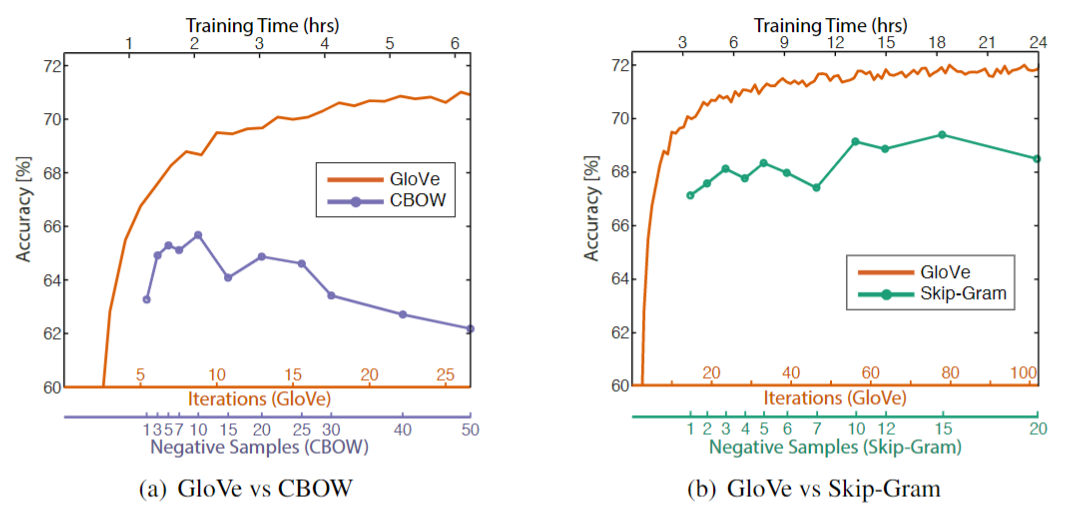
\includegraphics[width=0.8\textwidth]{imgs/table_gloveVSword2vec.png}
\vspace{-5pt}
\caption{\footnotesize Overall accuracy on word analogy task as a function of training time, which is governed by the number of iterations for GloVe and by the number of negative samples for CBOW (a) and skip-gram (b). Pennington et al. (2014) train 300-dimensional vectors on the same 6B token corpus from Wikipedia and use a symmetric context window of size 10. From \emph{GloVe: Global Vectors for Word Representation}, by Pennington et al., 2014. \url{https://nlp.stanford.edu/pubs/glove.pdf}. Copyright 2014 by Pennington et al.}
\vspace{-5pt}
\end{figure}